\documentclass{article}

\usepackage[margin=1in]{geometry} 

\usepackage{braket}
\usepackage[separate-uncertainty=true]{siunitx}
\usepackage{graphicx}
\usepackage{amsmath}
\usepackage{xurl}
\usepackage{titling}
\usepackage{algorithm}
\usepackage{algpseudocode}
\usepackage{mathtools}
\usepackage{amsfonts}
\usepackage{amssymb}
\usepackage{cprotect}
\usepackage{float}

\let\d\relax
\newcommand\d{\,\mathrm{d}}

\graphicspath{{./images/}}
\sisetup{range-phrase=\,--\,}


\begin{document}

\title{Machine Learning for the Detection of Frozen-In Crystallographic Defects in Solid Xenon \\[2.5ex] \large The University of Texas at Austin \\ Department of Physics}
\author{Evie Shear \\ Supervised by Scott Kravitz}
\maketitle
\pagebreak

\section*{Abstract}

One of the leading detector architectures in the field of dark matter detection is the dual-phase xenon time projection chamber (Xe-TPC): entering particles produce a detectable signal as they pass through a bath of liquid xenon. The use of Xe-TPC detectors such as LUX-ZEPLIN currently leads the world in bounds on the possible properties of WIMPs as a candidate for dark matter in the \qty{10}{\GeV/c^2} to \qty{100}{\TeV/c^2} mass range \cite{Aalbers2025}. However, the need to minimize radon background radiation has motivated the development of a new Xe-TPC model which utilizes xenon in a crystalline phase instead of liquid \cite{Kravitz2022}. Furthermore, this crystal must be highly regular to allow produced signals to pass through the xenon and arrive at the detector.

Using a database of images of crystalline xenon produced by the CrystaLiZe lab through freezing liquid xenon \cite{KravitzLabCrystaLiZe}, I developed a convolutional neural network (CNN) capable of detecting visually opaque freezes in xenon. The model is characterized by a ROC-AUC value of $\mathrm{AUC}=0.934$ for the validation data provided to it and an average total variation of $MTV_{seen}=12.8$ and $MTV_{unseen}=6.6$, indicating highly reliable performance on labeled data and low noise in the predictions of the model for both training/validation and unseen data. Furthermore, the model is able to predict poor-quality freezes significantly before the imperfections are visually apparent to the human eye and generalizes well on unseen data not used for training or validation given a fixed camera perspective.

\section*{Acknowledgments}

I would like to thank Professors Timothy Andeen, Vernita Gordon, and Scott Kravitz for helping me with the logistics of my thesis. A special thanks goes to Professor Kravitz for his guidance and support on this project and for giving me the environment to learn more about machine learning. I would also like to thank the members of the CrystaLiZe lab, especially Dr. Dan Hunt, for making the xenon freeze image database accessible to me and for helping with the day-to-day work. Lastly, I would like to thank my family and partner for being there for me when I needed them.

\section*{Background}

The nature of the phenomenon known as ``dark matter'' is one of the leading mysteries of high-energy physics and astrophysics today. Without dark matter, galaxies would not stay gravitationally bound together, and consequently it must take up around 5-6 times the total mass as regular matter, but its exact nature is a matter of ongoing debate and experimentation \cite{Aalbers2025} \cite{Bull2016}. One leading collection of hypotheses is that dark matter is composed of some type of weakly interacting massive particles (WIMPs).

These particles are detectable using a dual-phase xenon time projection chamber (Xe-TPC), depicted in Fig.~\ref{XeTPC}, which have set world-leading limits on possible WIMPs. When a high-energy particle enters the detector and interacts with the liquid xenon, it produces a light signal that is detected by a series of photomultiplier tubes at the ends of the detector. The high energy of the incoming dark matter particle also causes the liquid xenon to ionize, releasing electrons that accelerate when they reach the gaseous xenon and create an avalanche of secondary electrons and photons. The relative properties of these light pulses allow for the reconstruction of the high-energy particle/xenon interaction in space and time and for the characterization of the said particle's energy and interaction type (xenon nuclear interaction/electron recoil) \cite{Pushkin2019}.

\begin{figure}[h]
    \centering
    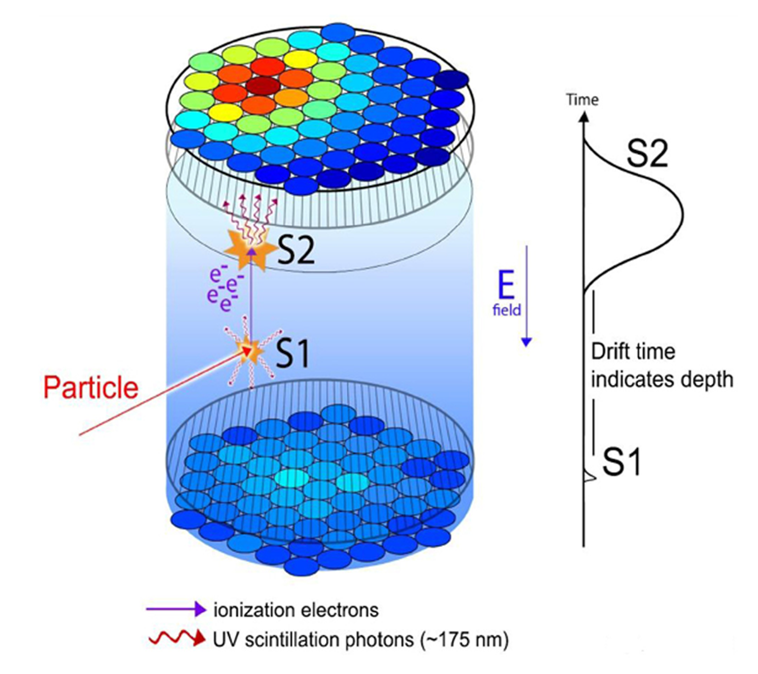
\includegraphics[width=0.8\textwidth]{XeTPC}
    \caption{Diagram of a dual-phase xenon time projection chamber (Xe-TPC). Shown is a dark matter particle (WIMP) moving from left-to-right, and interacting with the liquid xenon, causing it to ionize and scintillate, which releases light (S1) and electrons. These electrons drift upwards due to an electric field, and are absorbed by the xenon gas at the top, producing a second light signal (S2). Graphed along the right from bottom to top is the light signal vs. time detected by the PMTs at the top and bottom of the detector \cite{Pushkin2019}.}\label{XeTPC}
\end{figure}

A number of next-generation dark matter detectors currently use the Xe-TPC architecture, including LUX-ZEPLIN \cite{Aalbers2025} and XENONnT \cite{Aprile2023}. The primary obstacle to improving the sensitivity of these detectors is currently background radiation, mainly due to radon impurities. As uranium and thorium are present in trace amounts in detector materials, their decay product radon is able to enter the liquid xenon detector medium and produce background interactions that are difficult to discriminate from a true dark matter signal \cite{KravitzCWODS2026} \cite{Arthurs2021}. To combat this, the CrystaLiZe lab at UT Austin has been working to refine a Xe-TPC that uses crystalline xenon in place of the liquid form. The non-gaseous xenon being a solid rather than a liquid prevents the movement of atoms through its structure, and so excludes radon emitted by the detector as well as fixing spatially any radon daughter nuclei present in the crystal, allowing them to be tagged \cite{Kravitz2022} \cite{Pushkin2019}.

The xenon is frozen inside a cryostat (see Fig.~\ref{cryo}), where both a coldhead and heaters are present for controlled cooling of the system. Because the system can be both warmed and cooled at different ends, this allows for the creation of a temperature gradient throughout the cryostat which makes cleaner freezes possible. Inside the cryostat there are silicon photomultipliers (SiPMs) present in order to detect scintillation within the xenon media.

\begin{figure}[h]
    \centering
    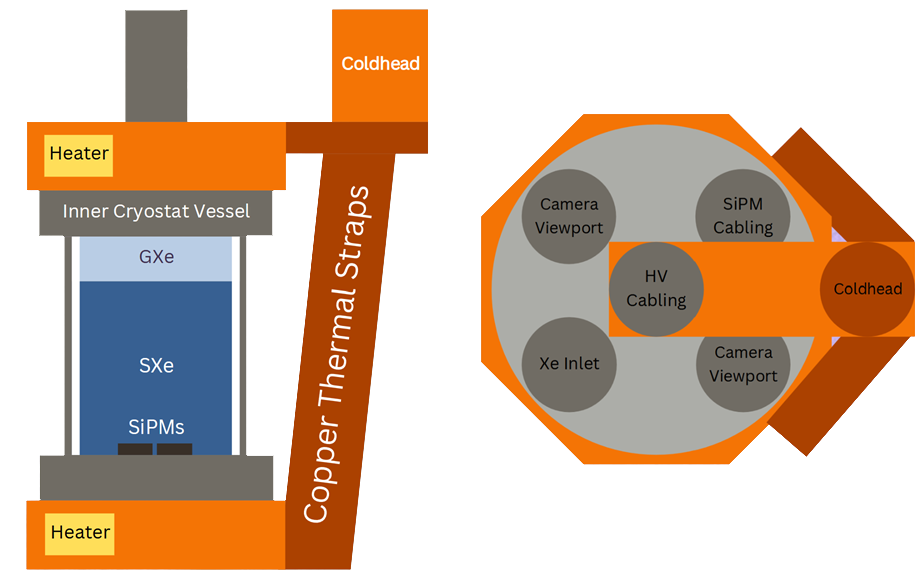
\includegraphics[width=0.8\textwidth]{cryo.png}
    \caption{Diagram of the cryostat containing the prototype xenon scintillation detector \cite{KravitzCWODS2026}. Left image depicts the cryostat from the side, right view depicts the cryostat from above. The coldhead and the heaters allow for the creation of a temperature gradient necessary for low-defect xenon freezes. Silicon photomultipliers (SiPMs) detect scintillation in the xenon media. Camera viewports look into the cryostat from above.}\label{cryo}
\end{figure}

\section*{Machine Learning}

\subsection*{Model Architectures}

As the xenon freezing process occurs around the clock, the status of the xenon freeze within the cryostat cannot be monitored at all hours of the day. Furthermore, partially frozen xenon crystals with imperfections tend to become more opaque over time. Through the use of a camera, we can automatically detect opacity in the visible spectrum, which is a generally indicative of for opacity in the UV range. Furthermore, opacity in the UV range then leads to absorption and loss of the particle signal (S1). Therefore, if we can use live camera data to respond to visual defects in the xenon automatically, it would make possible fixing poor xenon freezes around the clock in real time. In order to properly respond to visual crystallographic defects being ``frozen-in,'' I developed a machine learning model that is able to continuously monitor the xenon freezing process in order to notify a lab member and allow a rapid response when these defects begin to develop.

Machine learning is a rapidly expanding field focused on the automated development of algorithms that perform tasks that are highly difficult or resource intensive for humans to manually automate. To this end, a set of training data and labels is given to the model, from which it attempts to learn how to predict the label for a general data point to the best degree possible. In order to make sure that the model has learned the general pattern and not only the training data, it is given a set of validation data which is used to test its performance on a dataset it has not trained on.

My initial goal was to develop an algorithm that takes an image of the xenon medium in the detector and outputs a quality score Q: $Q=1$ if the xenon was visually frozen imperfectly, and $Q=0$ otherwise (i.e., the xenon is liquid or frozen without visual defects). Additionally, I wanted the model to have the following properties:
\begin{enumerate}
    \item Generalizability: The model should perform well on data it has never seen before,
    \item Forecasting: The model should be able to determine when a poor freeze is imminent significantly before a human could,
    \item Well-Behaved: The model should have low output noise over time and be monotonically increasing during a bad freeze.
\end{enumerate}
Item (1) is a goal for all machine learning models. Item (2) was motivated by the hypothesis that an algorithm should on average perform better than a human, as it can recognize more subtle patterns. Item (3) was motivated by the physical reality that freezing occurs over time, and that as the xenon gets more visually opaque, the model's prediction should correspondingly increase.

As the CrystaLiZe lab had a large database of images at the outset, the problem was to find what technique could best map visual properties onto desirable outcomes. To this end, two models were considered: a boosted decision tree (BDT) and a convolutional neural network (CNN). The former is a model frequently used on the classification of low-dimensional datasets, and the latter exploits the spatial properties of images to find relevant features in the image. While image data appears high-dimensional (many pixels, 3 color channels), it was plausible to me that a few general image properties could be extracted from an image from which a BDT could classify freezes.

For the BDT architecture, I used the python package \verb|XGBoost| \cite{XGBoostDocumentation}. A decision tree is a directed tree where starting from the root node, a given data point is sorted into one of several discrete categories based on its properties. For an example, see the tree in Fig.~\ref{DT}. Additionally, the leaf nodes of a decision tree, i.e., the farthest nodes from the root node, can also correspond to values of a continuous variable; this is the case for a tree in a BDT model, for which each leaf node of a single tree corresponds to some predicted value $\hat Q_i$ for the quality $Q \in [0,1]$. However, instead of using a single tree, a BDT recursively builds an ensemble of decision trees, procedurally using each new tree to improve on the prediction made by the ensemble up to that point. This allows a collection of trees which are individually weak classifiers to be combined into a single strong classifier.
\begin{figure}[h]
    \centering
    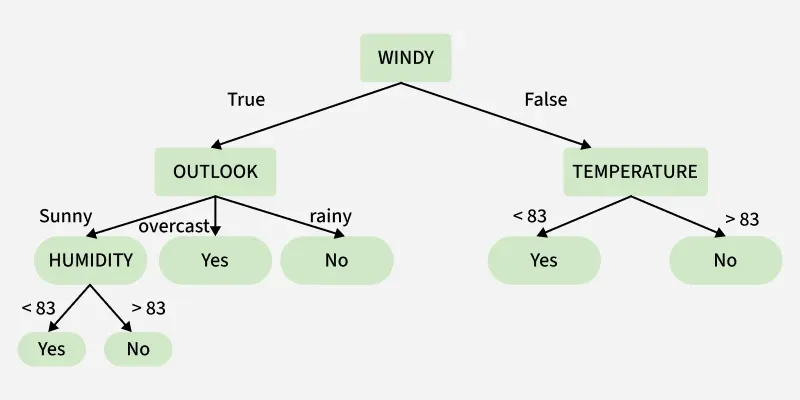
\includegraphics[width=0.8\textwidth]{DT.png}
    \caption{Example of a decision tree \cite{GeeksforGeeksDecisionTree}. Based on whether it is windy, the weather outlook, the humidity, and the temperature, it gives an answer of either ``yes'' or ``no'' to the question, ``Is it a nice day outside?'' For example, if it is windy and the outlook is overcast, the tree says that it is a nice day outside.}\label{DT}
\end{figure}

\verb|XGBoost| builds a BDT ensemble by first starting with the empty ensemble $E_0=\emptyset$ and the base prediction $F_0=f_0=p$, where $p$ is the probability that a uniformly randomly selected image has $Q=1$. The process is that at each recursion step $i$, a new tree $T_i$ is built and its prediction function for the residuals
\[f_i \approx Q_t-F_{i-1}(\text{Image}_t)\]
is added to the ensemble to obtain
\[F_{i}=F_{i-1}+f_{i}=\sum_{k=0}^{i} f_k,\]
where $Q_t$ is the true quality of $\text{Image}_t$. The tree $T$ associated with $f_{i}$ is optimized through the method of gradient descent, by which \verb|XGBoost| can decide where it may be optimal to add a new node or change the value of existing nodes. In other words, this allows new trees and nodes to correct the errors made by the previous ensemble. Once the tree reaches a certain number of leaves or depth, the tree finalizes and the algorithm moves on to the next tree $T_{i+1}$ \cite{GoogleGBDT}.

For a CNN architecture, I used the \verb|tensorflow.keras| python package \cite{TensorFlowDocumentation}. A CNN is a neural network containing a number of convolution layers followed by several dense layers. To unpack this definition, a neural network is an interconnected set of nodes with (directed) edges connecting them, designed to perform an analogous function to neurons and synapses in the human brain. Attached to the edges are quantities called weights, and attached to the nodes are biases. Nodes are organized into internally disconnected groups called layers; the output from a given layer is put through a linear transformation composed with an activation function to obtain the value of a node in the next layer. For example, if $\mathbf N$ are the nodes in the previous layer connected to the present layer $\mathbf N'$, $W_{ij}$ is the weight for the edge from $N_j$ to $N_i'$, $\mathbf B$ are the biases of $\mathbf N'$, and $r$ is some activation function, we find that
\[\mathbf N' = [\mathbf R(\mathbf W\mathbf N+\mathbf B)_j]_j,\]
where $\mathbf R(\mathbf v)= [r(v_j)]_j$ outputs the vector where $r$ is applied element-wise to a vector $\mathbf v$. Since a composition of linear transformations is linear, in order to capture non-linearity the activation function must not be linear, such as the ReLU function
\[\text{ReLU}: \mathbb R \to [0,\infty),\ \text{ReLU}(x)=\begin{cases}
    0; & x \leq 0 \\
    x; & x > 0
\end{cases}\]
or the sigmoid function
\[\sigma: \mathbb R \to (0,1),\ \sigma(x)=\frac{1}{1+e^{-x}}.\]
Gradient descent is then used to obtain a slightly ``better'' prediction function according to the metric of a loss function $l(Q, \hat Q)$, where $\hat Q$ is the predicted quality of a given image as a function of all the weights and biases of the network.

A layer is dense if the previous and current layer form a complete bipartite graph. A layer is convolutional if nodes from the previous layer are locally connected to the present layer via a translation invariant matrix, called a kernel. For example, suppose we have a 1 by 5 grayscale image with brightness values
\[I=\begin{bmatrix}
    0 & 1 & 0 & -1 & 2 \\
\end{bmatrix}\]
and a 1 by 3 kernel
\[K=\begin{bmatrix}
    -1 & 0 & 1
\end{bmatrix}.\]
We can slide this kernel over the image so that
\[I_j'=\sum_{k=-1}^1 I_{j+k}K_{k+2},\]
where we set $I_0=I_6=0$. Therefore,
\begin{gather*}
    I'=\begin{bmatrix}
        0\cdot (-1) & + & 0 \cdot 0 & + & 1 \cdot 1 \\
        0 \cdot (-1) & + & 1 \cdot 0 & + & 0 \cdot 1 \\
        1 \cdot (-1) & + & 0 \cdot 0 & + & (-1) \cdot 1 \\
        0 \cdot (-1) & + & (-1) \cdot 0 & + & 2 \cdot 1 \\
        (-1) \cdot (-1) & + & 2 \cdot 0 & + & 0 \cdot 1
    \end{bmatrix}^\intercal \\
    =\begin{bmatrix}
        1 & 0 & -2 & 2 & 1
    \end{bmatrix}.
\end{gather*}
This effectively connects each node and its 2 neighbors in $I$ to the corresponding node in $I'$, finding features in a 1 by 3 window in a manner that remains translation invariant over the whole image, both adding symmetry to the neural network and correspondingly reducing the number of parameters that need training.

Importantly, the spatial structure of the next layer is preserved: the relative positions of the convolved pixels in the next layer to each other are the same as the relative relation of the bounding boxes to each other in the previous layer. This grid of spatially organized convolved pixels in the following layer is called a feature map, as in optimal circumstances they extract relevant features from the given image in the convolution layer. Furthermore, there may be several unrelated feature maps (spatially related grids) in the next layer in order to extract multiple features. After a convolution layer, a CNN typically includes a downsampling layer in order to reduce weights, prevent overfitting, and extract the most relevant values from the feature maps. Finally, the convolution and downsampling layers are followed by several dense layers. The hyperparameters of the model such as numbers of layers and kinds of layers are all highly variable from problem to problem, and correspondingly are customizable using \verb|tensorflow.keras|.

\subsection*{Data Preparation}

\begin{figure}[h]
    \centering
    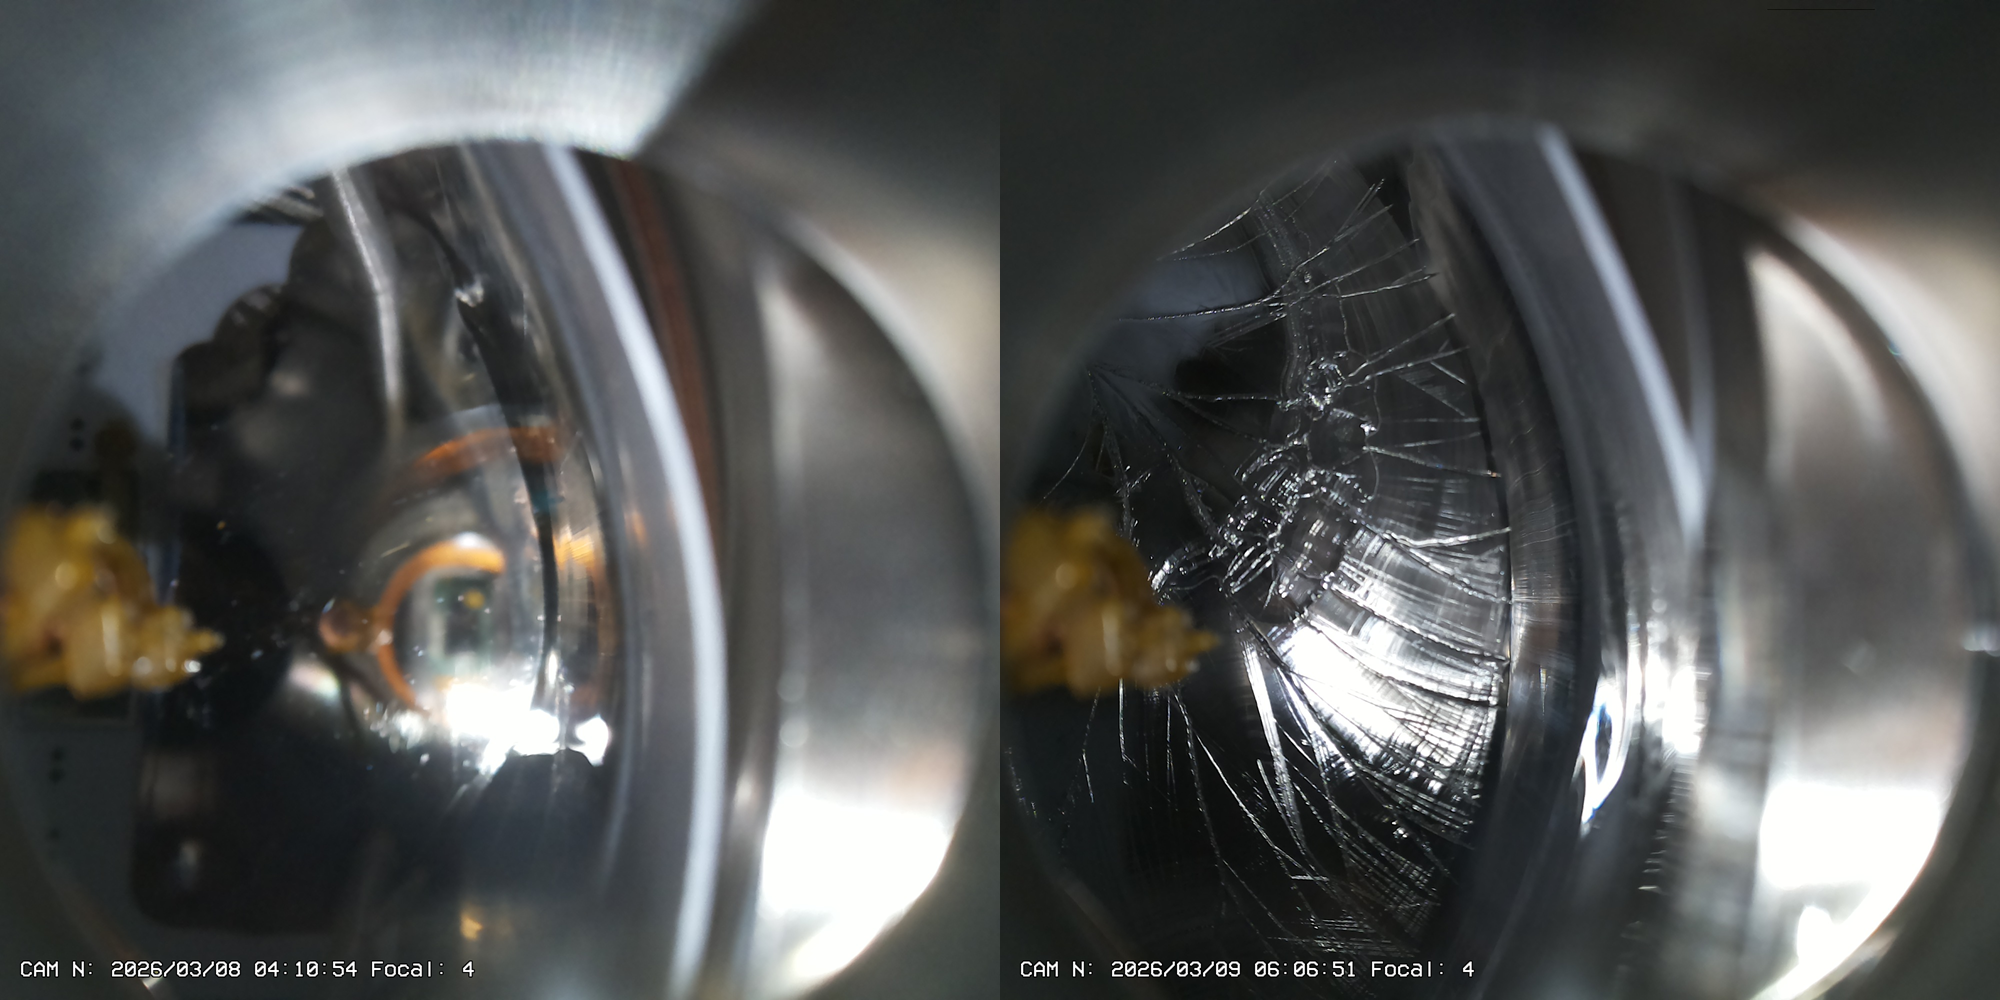
\includegraphics[width=\textwidth]{quality01.png}
    \caption{On the left is an example of an image with quality value close to 0 (not frozen or frozen transparently). On the right is an example of an image of quality value close to 1 (opaquely frozen). Both images were taken with a focal length of 4 (compare to Fig.~\ref{RQplots}).}\label{quality01}
\end{figure}

The images of the xenon (see Fig.~\ref{quality01}) were organized by timestamp and the focal length of the camera on Box, where the focal length of the camera determined whether the image's focus was further towards the bottom of the cryostat or the surface of the xenon. These images were taken in a way that their sequence at a given focal length closely approximates the appearance of the xenon in real time: roughly every two minutes, a photo is taken by the camera at even focal lengths from 0 to 10. Due to the total data comprising several terabytes, I utilized data about when freeze runs occurred and ended to determine the relevant time frames during which data was recorded that might be useful to the model, and then downloaded them to my local machine using a python script.

The first problem after I had obtained the data was classifying it by quality $Q$. Because of goal (2) (forecasting), I could not simply identify images in the $Q=0$ bin by eye, as I might identify a number of false negatives. Therefore, in order to determine when a phase shift occurred in the image properties, I modified code from a past lab member in order to plot several image metrics over time for each freeze run. The metrics used were the following:
\begin{enumerate}
    \item The standard deviation of an image. Measures the variance in the brightness of an image from pixel to pixel.
    \item The Shannon entropy of an image \cite{skimagemeasureDocumentation}. Used as another metric of the degree of variation of pixel brightness values.
    \item The variance in the Laplacian of an image \cite{OpenCVDocumentation}. Used as a metric of sharpness/blurriness of an image.
    \item The mean brightness of an image.
    \item The structural similarity index metric (SSIM) \cite{skimagemetricsDocumentation}. Used to identify the similarity of an image to a fixed qualiy 0 image.
\end{enumerate}
While the original images were 2000x2000 in RGB, these quantities were calculated on a grayscale version of the images downsampled to 500x500 to improve speed without losing substantial amounts of detail, as cracks in the xenon should still be visible at lower resolution and without color. I also stratified the plots of the data in Fig.~\ref{RQplots} by focus (different color points correspond to different focal lengths), and used timestamp as an independent variable. In these plots clear ``phases'' in image behavior can be observed that are shared across plots at a given timestamp. For example, until around 6am on 3/8, the plotted values are relatively constant. At this timestamp, there is a sharp change in slope and curvature on all plots except for that of the Laplacian variance, corresponding to the xenon visibly beginning to freeze.

\begin{figure}[h]
    \centering
    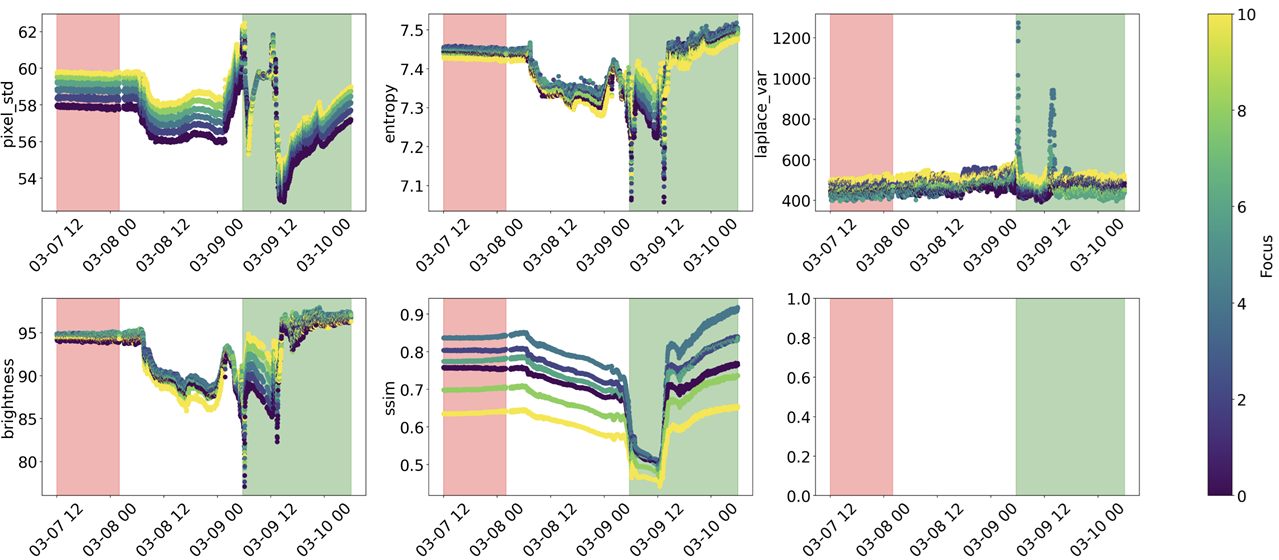
\includegraphics[width=\textwidth]{RQPlotsnew.png}
    \caption{Plots of image metrics of images from a freeze run lasting from 12pm on 3/7/2026 to 6pm on 3/10/2026. Data point colors are stratified by the focus of their corresponding image. Metrics (1)-(5) are plotted from left-to-right and top-to-bottom in reading order. The quality 0 time-range is highlighted in red, while the quality 1 time-range is highlighted in green. Different trends in the data can be seen in the green vs. red regions.}\label{RQplots}
\end{figure}

These plots can be compared to the example images from this freeze run in Fig.~\ref{quality01}. As can be seen, these images differ substantially both visually and according to their image metrics seen in Fig.~\ref{RQplots}. However, since the image metrics are non-monotonic (e.g., many images in the quality 0 region share the same brightness with some images in the quality 1 region), no one of these image metrics is sufficient to determine the image quality. This makes determining the quantitative properties corresponding to a specific image quality a difficult task to perform manually.


Looking at the images, I was unsure which of these phases corresponded to poor freezing and which corresponded to regular freezing, as it was possible that images show signs of poor freezing before a human would know what to look for. While I ended up with a combination of supervised learning with a meta-evaluation of the appropriateness of a model architecture using unlabeled data of ambiguous quality, both unsupervised and semi-supervised learning could potentially have been used here in order to deal with the data of ambiguous quality. However, ultimately I chose the method I used based on the time constraints of this project combined with the additional structure that timestamping gave to the images I did not label with a quality. However, a future project that utilizes these styles of machine learning would allow for further exploration of these areas.

Therefore, I decided that the safest option would be to take blocks of time for images of a given quality: all images in the chronologically first phase would be quality 0, and all images after the xenon turned visibly opaque (corresponding to a poor freeze) would be quality 1. All data in between these times would not be labeled and so neither trained nor validated on, but would be used to judge the performance of the finished model based on the three properties mentioned above.

\begin{figure}[H]
    \centering
    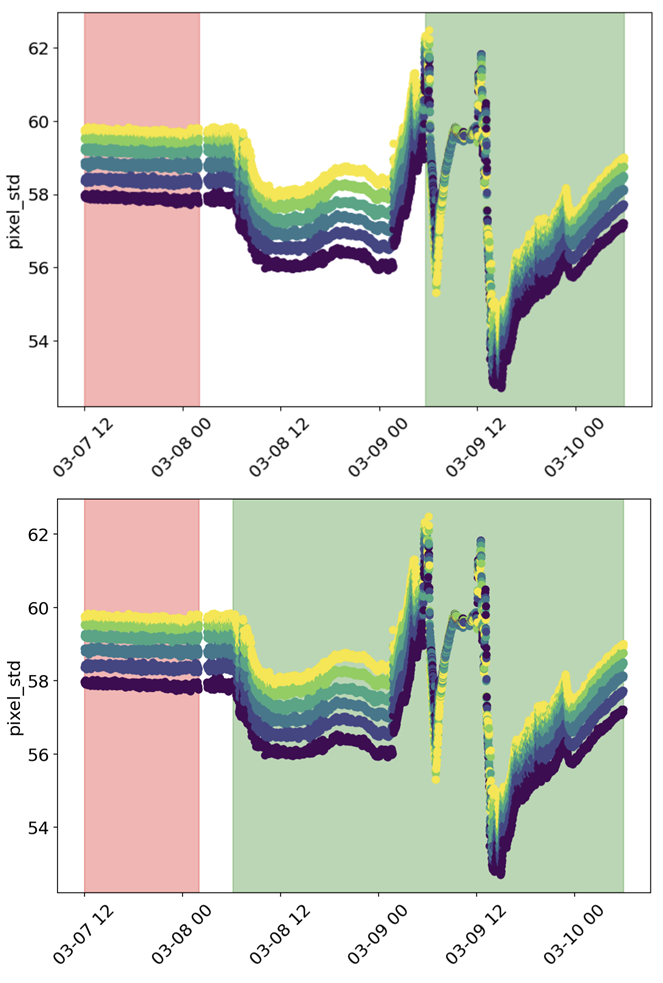
\includegraphics[width=0.8\textwidth]{pixelstdRQs}
    \caption{Time ranges for quality labels overlaid over a plot of image standard deviation vs. time. Focal length corresponding to images are labeled by the color bars in Fig.~\ref{RQplots}. Red time ranges denotes quality 0, while the green time ranges denote quality 1. The top plot shows the intended labeling used for validation; the bottom plot shows the labeling used for training.}\label{pixelstdRQs}
\end{figure}

This gave me approximately 22900 images to work with, or around 3800 of each focal length. However, at some point in the process these timestamps were mislabeled, and some of the intermediate images made it into the labeled images. An example of this is given in Fig.~\ref{pixelstdRQs}. For the corresponding 3/9 freeze run, I successfully labeled the quality 0 images, going from the start of the freeze to the point where the flat line on the plot starts to tilt slightly upward. However, I labeled the start of the quality 1 images far too early, as the freeze only appeared visibly bad to me at 6am on 3/9. While the $Q=1$ time range is not what I originally intended, there was not sufficient time to fully explore the effects of this mislabeling, other than that 749 out of 2045 images were mislabeled as quality 1 from the ``0309'' freeze run, and 143 out of 626 were mislabeled as quality 0 from the ``0318'' freeze run. Additionally, this mislabeling was only used during training and not during the following analysis. However, I will give some further details on the effects of this mislabeling further below.

\section*{Development and Analysis}

\subsection*{Boosted Decision Trees}

For the BDT, I developed two models. The first model took in the five properties of a single image enumerated above, considering only a single focal length. The second model took in the qualities of consecutive groups of 6 images, one of each focal length. The motivation for this second model was that different image foci are not truly independent but rather captured image data at different distances from the camera. Thus, since groups of 6 images are taken chronologically close to each other, a cluster of images taken with different foci would hypothetically give a better picture of what was occurring than any one focus.

These models were created using \verb|XGBClassifier| and scikit-learn's \verb|GroupKFold|. \verb|XGBClassifier| initializes the BDT with hyperparameters given in Table~\ref{BDTHyperparameters}: I set \verb|max_depth| and \verb|learning_rate| to be low to minimize overtraining, and \verb|n_estimators| at an appropriate value for the given learning rate to make sure learning occurs without overtraining. \verb|GroupKFold| allows me to cross-validate the data through setting each freeze as a validation dataset for a different model; as the images taken at closely spaced time intervals tended to be very similar, if data from a single freeze was used for both training and validation, the ability of the model to generalize would not be appropriately tested. Plotted in Fig.~\ref{BDT-AUC} are the ROC curves for these two models and the corresponding ROC-AUC (area under the curve) values.

\begin{table}[h]
    \centering
    \cprotect\caption{\verb|XGBClassifer| hyperparameters}
    \label{BDTHyperparameters}
    \begin{tabular}{c|c}
        Name & Value \\
        \hline
        \verb|n_estimators| & 300 \\
        \verb|max_depth| & 4 \\
        \verb|learning_rate| & 0.05 \\
        \verb|subsample| & 0.8 \\
        \verb|colsample_bytree| & 0.8 \\
        \verb|random_state| & 42 \\
        \verb|eval_metric| & ``logloss''
\end{tabular}
\end{table}

The ROC curve is calculated as follows: for each data point the model gives a quantity $q_1 \in [0,1]$ that the model attempts to relate to the true image quality $Q \in [0,1]$ in a monotonically increasing way. If we set a threshold quantity $q$ and assume that all images where $q_1 > q$ are quality 1 and all images where $q_1 < q$ are quality 0, this gives a number of true positives ($TP$), false positives ($FP$), true negatives ($TN$), and false negatives ($FN$). The true positive rate $TPR$ is
\[TPR(q)=\frac{TP(q)}{TP(q)+FN(q)}=P[q_1 > q \mid \text{Predict}(\text{Image}_{q_1}) \text{ is correct}],\]
and the false positive rate $FNR$ is
\[FNR(q)=\frac{FP(q)}{FP(q)+TN(q)}=P[q_1 < q \mid \text{Predict}(\text{Image}_{q_1}) \text{ is incorrect}],\]

\begin{figure}[H]
    \centering
    
\includegraphics[width=0.8\textwidth]{BDT-AUC.png}
    \caption{ROC Curves and ROC-AUC values for the combined predictions of all BDT cross-validation models. The top image was created using the cross-validation predictions of the BDT with standalone image data (no grouping by focal length) as inputs. The bottom image was created using the cross-validation predictions of the BDT with groups of images of varying foci as inputs.}\label{BDT-AUC}
\end{figure}

where ``Predict(Image)'' returns either $Q=0,1$. Then the ROC curve can be obtained using the parameter $q \in [0,1]$ by plotting
\[ROC(q) = \Big(FPR(q), TPR(q)\Big) \in [0,1]^2.\]
ROC curves for more predictive models have higher values for the AUC and are a smaller distance from the point (0,1) \cite{TDSROC}; for example, for a random predictor the TPR equals the FPR, so
\[AUC_{random}=\int_0^1 TPR(FPR)\d(FPR)=\int_0^1 x\d x = 0.5,\]
and for a perfect predictor either $FPR=0$ or $TPR=1$ so that
\[AUC_{perfect}=\int_0^1 \d x=1.\]


From this it can be seen that both models do fairly poorly, and the model that takes in groups of image data does not do significantly better than randomly guessing. Plotted in Fig.~\ref{BDTPlots} are the predictions of these two models on a dataset not included in the training or validation data. This shows that the models do not have any of the 3 properties I was looking for, as none of (1), (2) or (3) apply to the predictions on this dataset.

\begin{figure}[h]
    \centering
    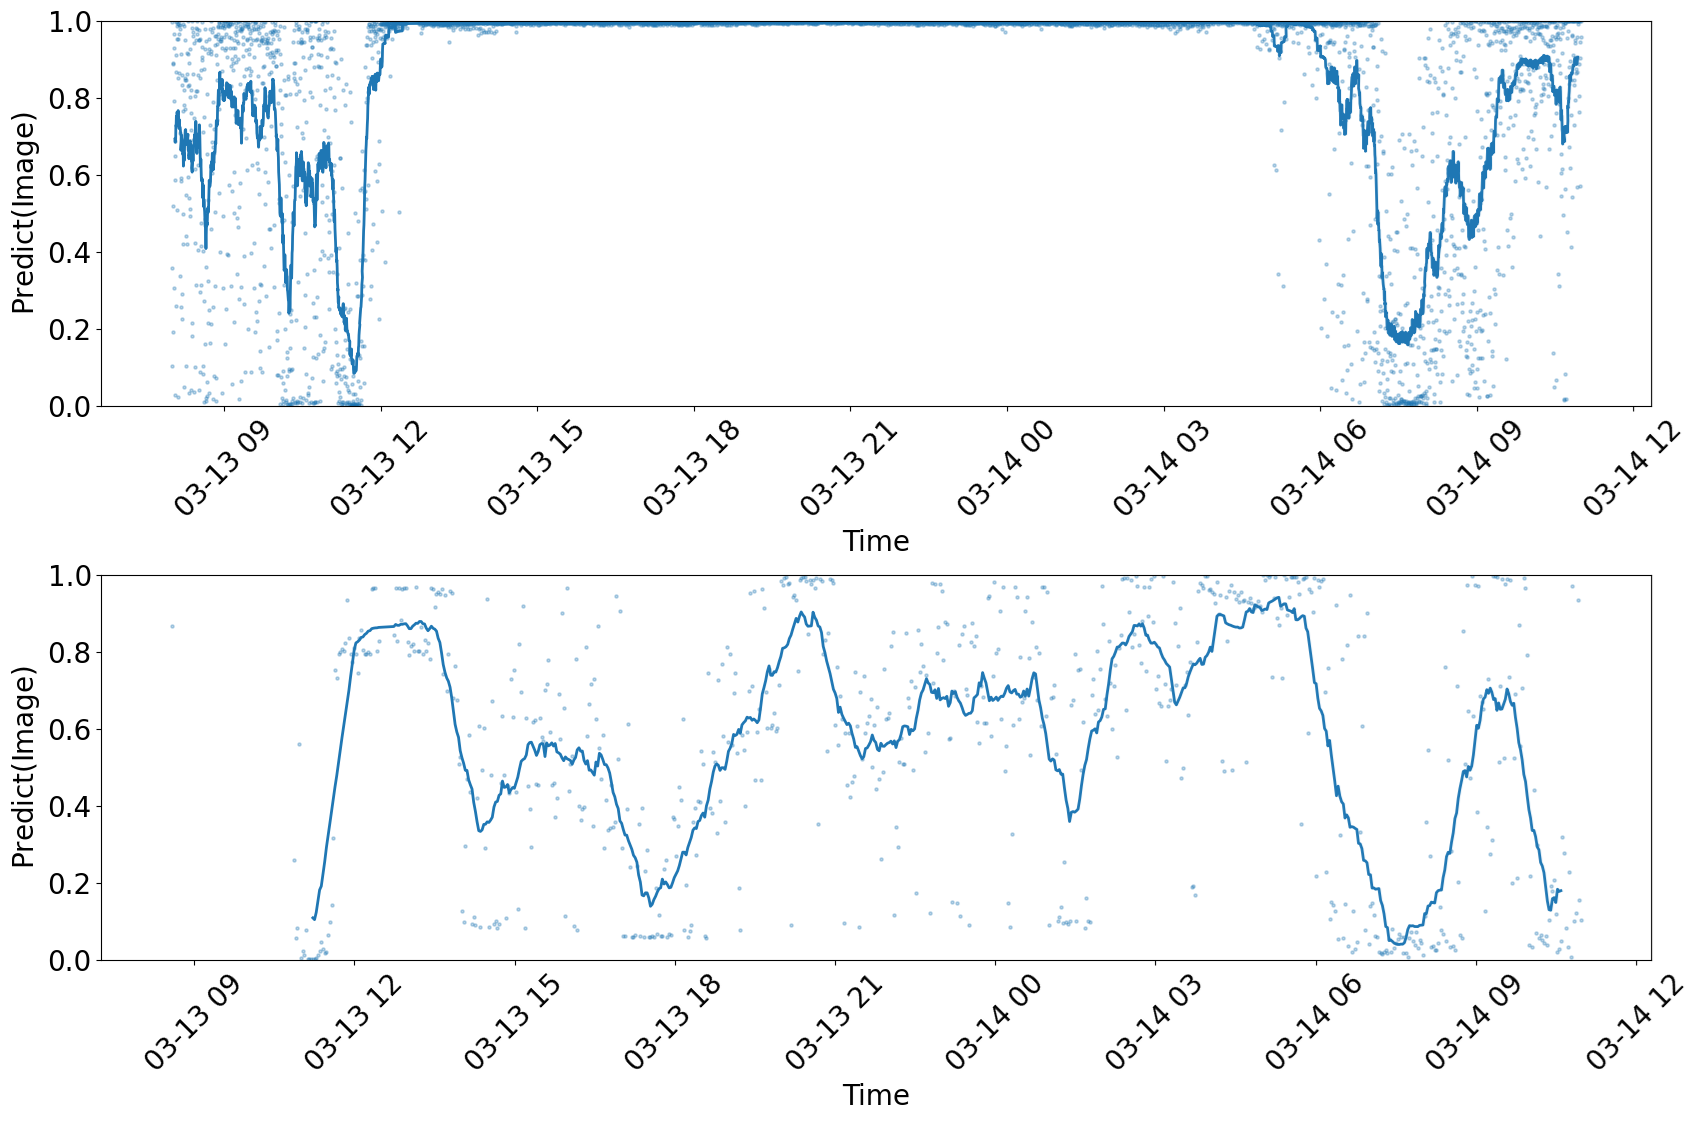
\includegraphics[width=\textwidth]{BDTPlots.png}
    \caption{Plots of the predicted qualities for an unlabeled dataset not trained or validated on by the 2 BDT models. The individual data points are plotted as a scatterplot, and the blue curve is the average of the last 25 data points in order to introduce smoothing. The top plot was created using the cross-validation predictions of the BDT with standalone image data as inputs. The bottom plot was created using the cross-validation predictions of the BDT with groups of images of varying foci as inputs.}\label{BDTPlots}
\end{figure}

\subsection*{Convolutional Neural Networks}

\subsubsection*{Development}

Due to these decisions for the model architecture leading to poorly predictive models, I made several decisions going forward. First, I would stick to one focus so that the model might learn how to predict for a single focus better than if it has to predict well for multiple foci. Furthermore, I found that the focus $f=4$ is where the cracks in the xenon became most easily visible to me, and so I decided to use this focus. Secondly, I decided to see if a CNN would function better, as I was seeing poor results so far for the BDT architecture. However, a difficulty with this model I ran into was that a CNN needs a much larger amount of training data than a BDT typically does due to the large number of weights for the model (a good rule of thumb is to have more training data points than trainable parameters). Given that I had 3815 images and that the number of weights in a CNN scales like the image side-length squared, with a 500x500 image a single convolution layer already has at least 250k weights. Thus, I had to find several ways to work around this issue.

The first way I addressed this problem was decreasing the resolution of the images in order to decrease the number of weights needed for the convolutional layers. First, I cropped the largest square I could create in the image that contained solely the xenon in order to remove extraneous data. Secondly, I downsampled the images: I started out with 64x64 images (see Fig.~\ref{64x64_q01}), but later experimented with 96x96 images. The second way I addressed the above problem was data augmentation: using the data I already had and slightly modifying it to create additional data. For each image, I created 4 images that had been randomly flipped (horizontally and/or vertically) and rotated, and then used those 4 images as data, effectively quadrupling my dataset. An additional plus to this process is that it potentially creates greater invariance of the model's predictions to linear transformations. Finally, I kept the number of layers in the model fairly shallow in order to reduce the number of weights contributed by the depth of the network (see Fig.~\ref{NNBlockDiagram} below).

\begin{figure}[h]
    \centering
    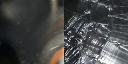
\includegraphics[width=\textwidth]{64x64_q01.png}
    \caption{Examples of 64x64 RGB image data used for CNN training/validation. Depicted are images of quality 0 (left) and quality 1 (right). Note that the cracks and opacity of the crystal on the right are still apparent at this resolution (compare to Fig.~\ref{quality01}).}\label{64x64_q01}
\end{figure}

As stated above, training a CNN involves feeding it data and it performing gradient descent on its weights and biases using this data. In this case, it trains on a whole randomly augmented dataset, and after a round of training (called an epoch), it trains on a newly randomized version of that dataset. To create the model, I initially used the following design:
\begin{enumerate}
    \item Using \verb|GroupKFold| to cross-validate using separate freezes for validation data,
    \item Using several callbacks: 
    \begin{enumerate}
        \item Stopping the model early each epoch if it starts overfitting to the data (i.e., if validation loss significantly decreases),
        \item Saving a model if a new record validation loss value is reached,
        \item Slowing training rate if the model approaches a minimum in parameter-space,
    \end{enumerate}
    \item Training for 100 epochs with the model architecture seen in Fig.~\ref{NNBlockDiagram}.
\end{enumerate}

\begin{figure}[h]
    \centering
    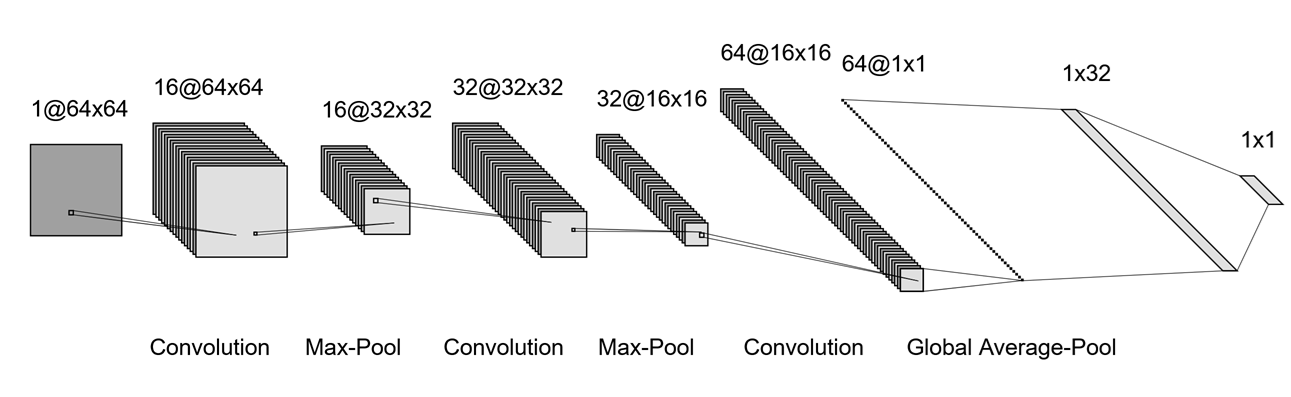
\includegraphics[width=\textwidth]{NNBlockDiagram.png}
    \caption{Block diagram of the initial architecture used for the CNN model. Each 2D layer is labeled above with the number of feature maps followed by the resolution and below with the operation name. The last two layers are dense layers with a dropout of 0.5 between the penultimate and final layer.}\label{NNBlockDiagram}
\end{figure}

All the convolutional layers used a 3x3 kernel. The convolutional layers and the first dense layer used the ReLU activation function, while the final dense layer uses a sigmoid activation function in order to normalize the output to a value between 0 and 1. The sequence of convolutional layers having an increasing number of feature maps is because, firstly, the max pooling layers reduce the number of nodes by a half, so more feature maps can be added without adding too many parameters, and secondly, more feature maps at deeper layers can allow for higher levels of abstraction from the layers closer to the input, which can only look at local features like edge detection. The max pooling layers take the highest value in a 2x2 block to find the most important features (largest node activations), reduce overfitting, and allow for some translation invariance \cite{Lecun1998}, while the global average pooling layer also reduces overfitting while also greatly reducing the number of parameters needed by reducing each feature map to its average value in order to extract a single quantity for each feature in the final convolutional layer. The dense 32 node layer allows for classification based on the presence of the given features in the previous layer, and the dropout randomly sets half the values of this layer to zero in order to prevent overfitting (see Fig.~\ref{CNNperformance}) and increase the resilience of the network. Finally, the last layer serves as the output.

\begin{figure}[h]
    \centering
    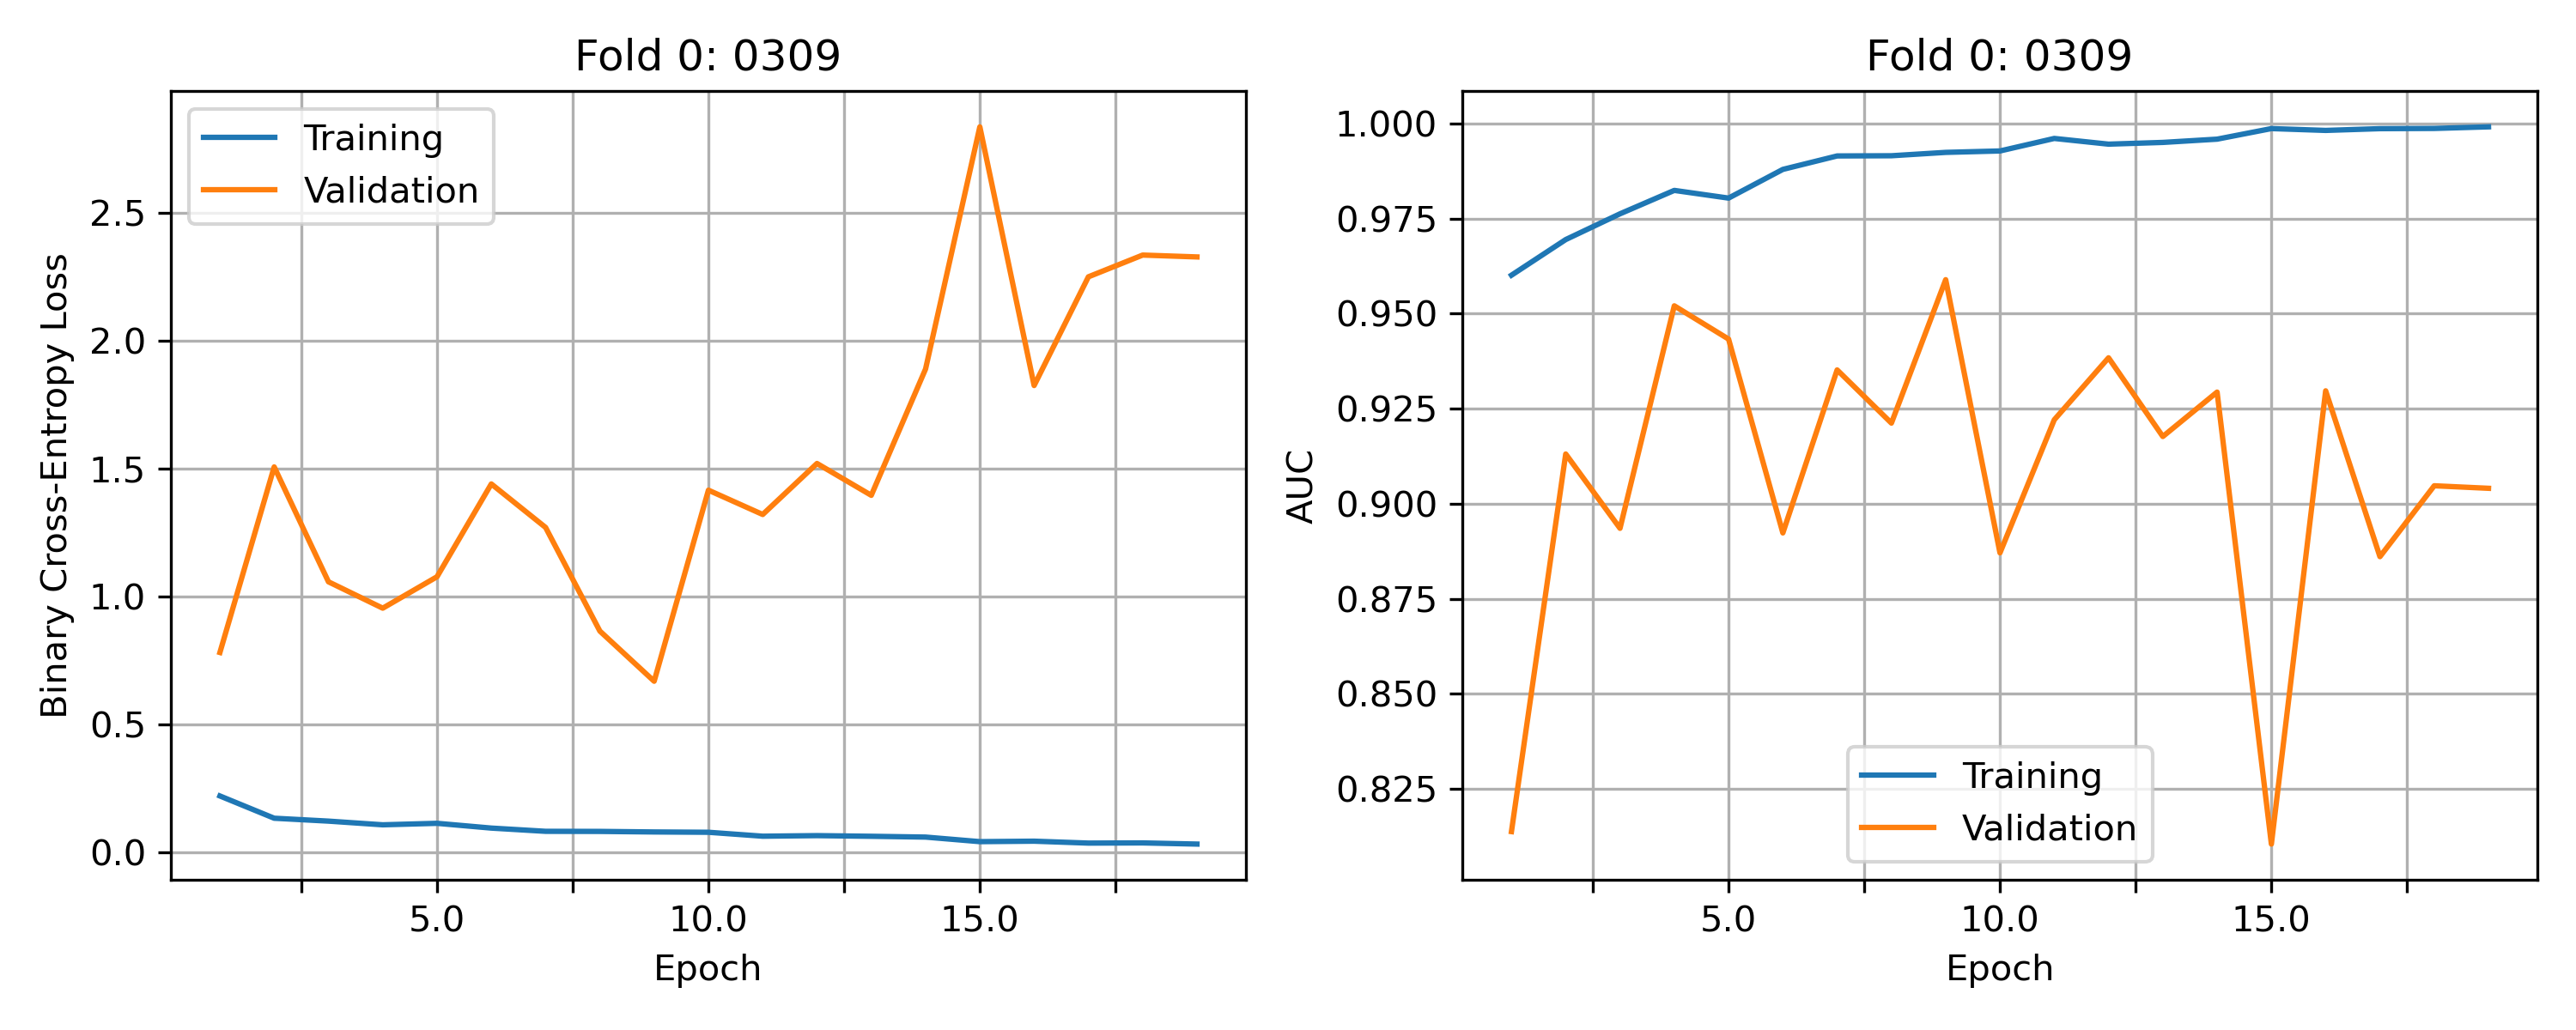
\includegraphics[width=\textwidth]{CNNperformance.png}
    \caption{Example of the loss and ROC-AUC of a model on fold ``0309'' across training epochs. Overfitting can be seen to occur beginning around generation 10, i.e., increasing validation loss and decreasing validation ROC-AUC, causing early stopping due to a callback.}\label{CNNperformance}
\end{figure}

Ultimately, I created 6 generations of models. The zeroth had no cross-validation, which was added in the first generation. The second generation added data augmentation, and so only generations two through five had all intended features. The third generation added 3 channels (RGB instead of grayscale), and so I decreased the resolution to 64x64 to compensate for the increased necessary parameters. As I saw improved results from this model, further models build upon this one. The fourth generation added two things: firstly, I attempted to increase the stability of the model by introducing small random changes to training image brightness and contrast. Secondly, I introduced batch normalization, which sets each set of neurons in a layer to have a mean value of 0 and standard deviation of 1 (modifiable by trainable parameters). This theoretically allows for more stable training by smoothing the parameter landscape \cite{Santurkar2018}. This generation performed worse than the previous, and so I returned to the model of generation three and added weight decay and switched from the Adam optimization algorithm to AdamW, which functions better with weight decay. Weight decay is another regularization method that penalizes large weights, and correspondingly decreases large weights over training epochs if they remain large \cite{Loshchilov2017}. These results were predictive of the data, but less so than the best generation three model, corresponding to the idea from generation four that training regularization is not what is needed to improve on generation three. Indeed, the literature supports the idea that training regularization does not significantly improve results for small data sets compared to just data augmentation \cite{HernandezGarcia2018}.

\begin{figure}[H]
    \centering
    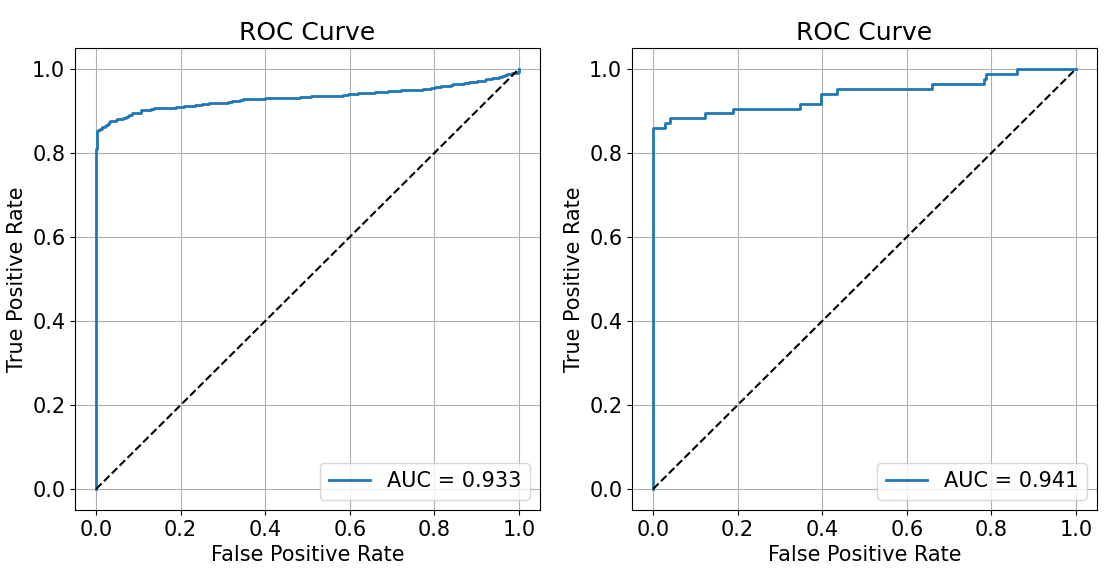
\includegraphics[width=\textwidth]{ROCcurves.png}
    \caption{Plots of the ROC curves for the CNN models III and Vb (left and right, respectively).}\label{ROCcurves}
\end{figure}

\subsubsection*{Analysis}

I used several metrics in order to determine the performance of these models: the ROC-AUC value, the mean total variation (MTV, defined below) of the model on training and validation data ($MTV_{seen}$), and the MTV of the model on data it has never seen before ($MTV_{unseen}$). Firstly, the ROC curve and ROC-AUC values were used in order to determine the overall performance of the model on data that I have explicitly characterized. The ROC-AUC values for the five working models I developed are given in Table~\ref{metrics}. Note that model IV's ROC-AUC value is 1.000 because the dataset it used for validation was extremely small, and not because it performs well in general. Displayed in Fig.~\ref{ROCcurves} are the ROC curves corresponding to the two highest ROC-AUC values (other than model IV), model III and model Vb. They are highly similar, but the curve for model Vb is slightly closer to (0,1) on the plot. Note that model Vb's ROC curve is less smooth as its validation dataset had fewer images.

\begin{table}[h]
    \centering
    \caption{Metrics characterizing viable CNN models. MTVs given in \unit{\percent\per\min}.}
    \label{metrics}
    \begin{tabular}{c|c|ccc}
        Model Generation & Changes & ROC-AUC & $MTV_{seen}$  & $MTV_{unseen}$ \\
        \hline
        II & 96x96 grayscale & 0.929 & 11.0 & 10.8 \\
        III & 64x64 RGB & 0.933 & 12.8 & 6.6 \\
        IV & BatchNorm + Augmentation & 1.000 & 46.5 & 30.6 \\
        Va & Weight Decay + AdamW & 0.902 & 21.8 & 14.4 \\
        Vb & Weight Decay + AdamW & 0.941 & 22.8 & 15.4
\end{tabular}
\end{table}


\begin{figure}[h]
    \centering
    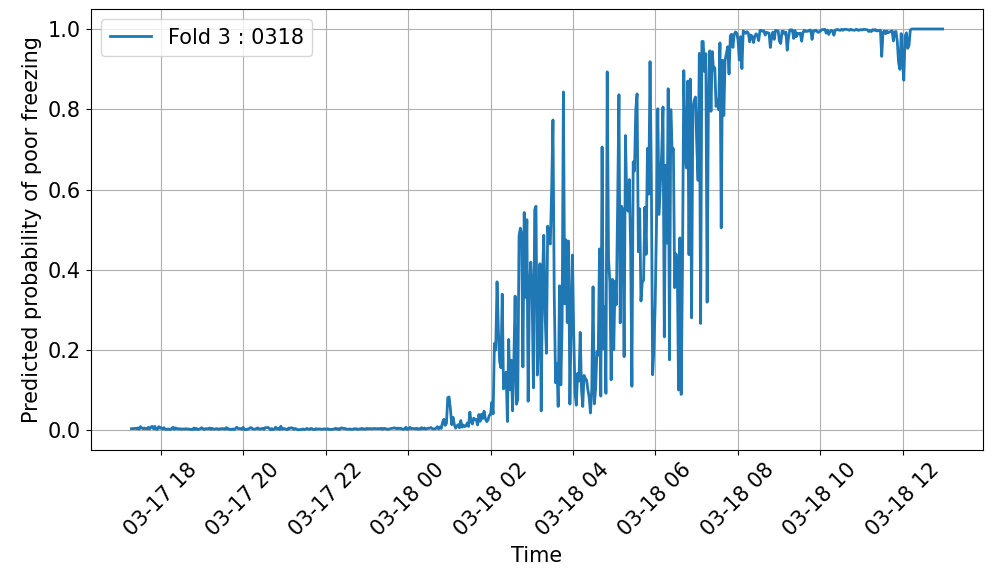
\includegraphics[width=0.8\textwidth]{modelIVPlot.png}
    \caption{Plot of the output of CNN model IV for the ``0318'' freeze run. Large amounts of noise dominate the output of the CNN.}\label{modelIVplot}
\end{figure}

In order to check which models satisfy desired property (3) (i.e., well-behavedness), I used the MTV, given by
\[MTV=\frac{1}{\# \text{ of runs}}\sum_i |\text{Predict}(\text{Image}_{t_{i+1}})-\text{Predict}(\text{Image}_{t_i})|,\]
where $\text{Predict}(\text{Image}_t)$ is the model's output in the range $[0,1]$ given the image at time $t$. Note that if a model is monotonically increasing on all data, it should have an MTV exactly equal to 1, since in each run it must transition from quality 0 to quality 1. Therefore, an MTV closer to 1 represents a signal-to-noise ratio closer to 1 (not accounting for transparent re-freezing over opaque freezes). The values for these quantities for each model are also given in Table~\ref{metrics} as $MTV_{seen}$, where the MTV is taken over the validation and testing data. Even though model IV has nearly as high an AUC value as model III, its $MTV_{seen}$ is much higher, and so it is not well-behaved. This can be seen in Fig.~\ref{modelIVplot}, where the amplitude of noise frequently dominates the output of the model. Additionally, model Vb performs better than model III according to the AUC value, but is significantly more noisy than model III, having a $MTV_{seen}$ of \qty{22.8}{\percent\per\minute} compared to model III's \qty{12.8}{\percent\per\minute}. This shows that the signal to noise ratio of model III's predictions is significantly closer to 1 than model Vb's. Additionally, we can see from the data that model II performs less noisily than model III on data that the modedl has seen.

Similarly, the MTV can be used to check property (1) (generalizability) by applying it to a freeze run that was not in the dataset used to test and validate the models, and correspondingly could not have affected the models' development. These values for $MTV_{unseen}$ are also given in Table~\ref{metrics}. As we can see, model III is the least noisy on new data, followed by model II. However, since my goal was to get a model that is both accurate and stable, I found that model III seemed to perform the best on average for my purposes according to these metrics.

\begin{figure}[h]
    \centering
    
\includegraphics[width=\textwidth]{CNNplotsnew.png}
    \caption{Plots of the predictions CNN models II (top), III (middle), and Vb (bottom) on freeze runs ``0309'' (left) and ``0302'' (right). The validation folds for the three models are runs ``0309,'' ``0309,'' and ``0506,'' respectively. Timestamps with images of quality 0 are highlighted in red, while timestamps with images of quality 1 are highlighted in green. Model II on run ``309'' jumps up to a prediction of 1 sharply when the quality label I provided switches to 1; it is unclear whether or not the model has ``cheated'' on its validation fold somehow or if it has not adequately learned how to forecast when an opaque freeze will occur and only learned what an opaque freeze broadly looks like.}\label{CNNplots}
\end{figure}

However, in order to check approximate monotonicity and property (2) (forecasting), I inspected the plots of the predicted quality over time for the models visually. As models II, III, and Vb are models that place first in some metric, these are the plots I most closely inspected.  For run ``0309'' (plotted in Fig.~\ref{CNNplots}, left), it can be seen that model III is the most monotonic and has the lowest noise. Interestingly, the xenon during this run only freezes visibly at around 3/9 at 6am, so model III seems to forecast this behavior. As this was the validation freeze for III, a potential explanation for this phenomenon is that I included a callback to stop training if the loss rose too much: because I mislabeled the start of the quality 1 timestamp block as 3/8 at 6am, the model may have been prevented from learning that the xenon only freezes opaquely later than this. However, the model begins to predict that the images are quality 1 starting over 12 hours after the faulty timestamp, so it is possible the model has actually learned to predict the freeze itself. This is reinforced by its behavior starting around 3/10 at 12am, where the xenon begins to freeze over the poor freeze cleanly, and correspondingly the prediction begins to decrease. Based on the fact that this specific decrease appears in all three displayed models, it seems likely that they all have learned to a better or worse degree what both a poor and good freeze looks like, and not just what freezing looks like in general. Run ``0322'' (not depicted) is two separate time chunks with images missing in between, both of which are quality 0, so all three models do well on this run. Only the quality 1 section of run ``0214'' (not depicted) was labeled, as the xenon starts this run with visible cracks in it, explaining the peaks at the start of the run in all three model's predictions. Model II performs the worst on run ``0318,'' (not depicted) both decreasing and increasing sharply. It is unclear which of III and Vb perform better on this run, as they both have significant noise. All three models perform poorly on run ``0506,''(not depicted) likely caused by significant movement of the camera taking images of the xenon. Lastly, for the unseen and unlabeled freeze run ``0302'' (plotted in Fig.~\ref{CNNplots}), model III performs by far the best, having extremely high monotonicity and low noise, especially compared to II and Vb. All these things (save potentially for its performance on run ``0318'') combined with its high performance in the metrics established above lead me to conclude model III is the best model, and can likely predict and identify poor freezes.

\section*{Conclusion}

In this thesis I developed multiple machine learning models to detect poor freezes in xenon for the purposes of building a new kind of dark matter detector, a dual-phase xenon time projection chamber using solid instead of liquid xenon. First, I developed two boosted decision tree models using 5 image metrics as inputs. Both of these models did not perform significantly better than random guessing, and did not meet the conditions of (1) generalizability, (2) forecasting, and (3) well-behavedness established above. In order to provide more potentially useful image data to a model, I switched to a convolutional neural network architecture, for which I built six models. Among these six, three warranted further examination, all of which perform well on the metrics of ROC-AUC and MTV, which indicates the accuracy of model predictions and smooth changes over time, as is desired for potential application as a automated alarm for poor freeze behavior. Examination of their predictions suggests all three models have learned how to predict poor freezes to a better-or-worse degree, among which model III performs the best in terms of properties (1)-(3).

For further research, data from more freeze runs would allow the model to refine its predictions and generalize further. Additionally, the data shows that the best models I developed are not able to predict freezes in general setups, and are highly sensitive to camera placement. As such, more freeze runs may allow for generalization to other camera placements or detectors. It is possible that using a pre-trained model with larger amounts of data as a base could generalize more easily based on the data available. It may also be possible to utilize machine learning optimized for time series to incorporate the sequential nature of images into the model's predictions for better noise prevention and stability over time. Similarly, additional metrics could be incorporated into predictions such as the pressure and temperature of the system. In terms of implementation, the algorithm needs to be integrated into a monitoring system for xenon freezes which can either modify freeze settings on the fly to correct poor freezes or notify a lab member so that they can manually do so if necessary. Another necessary aspect of future research is the application of the model: enough freeze runs need to be conducted in order to get statistical validation for the viability of the model's forecasts. Finally, the model's predictions could be compared with data and models of the xenon crystal structure in order to determine relative causes and effects for optical loss due to defects in the crystal structure.

All the code written by me for this thesis can be found on my GitHub \cite{EvieGitHub}.

\bibliographystyle{unsrt}
\bibliography{references}

\end{document}